\documentclass[letterpaper,11pt]{article}
\oddsidemargin -1.0cm \textwidth 17.5cm

\usepackage[utf8]{inputenc}
\usepackage[activeacute,spanish, es-lcroman]{babel}
\decimalpoint
\usepackage{amsfonts,setspace}
\usepackage{amsmath}
\usepackage{amssymb, amsmath, amsthm}
\usepackage{comment}
\usepackage{float}
\usepackage{amssymb}
\usepackage{dsfont}
\usepackage{anysize}
\usepackage{multicol}
\usepackage{enumerate}
\usepackage{graphicx}
\usepackage[left=1.5cm,top=2cm,right=1.5cm, bottom=1.7cm]{geometry}
\setlength\headheight{1.5em} 
\usepackage{fancyhdr}
\usepackage{multicol}
\usepackage{hyperref}
\usepackage{wrapfig}
\usepackage{subcaption}
\usepackage{siunitx}
\usepackage{cancel}
\usepackage{mdwlist}
\usepackage{svg}
\pagestyle{fancy}
\fancyhf{}
\renewcommand{\labelenumi}{\normalsize\bfseries P\arabic{enumi}.}
\renewcommand{\labelenumii}{\normalsize\bfseries (\alph{enumii})}
\renewcommand{\labelenumiii}{\normalsize\bfseries \roman{enumiii})}


\begin{document}

\fancyhead[L]{\itshape{Facultad de Ciencias F\'isicas y Matem\'aticas}}
\fancyhead[R]{\itshape{Universidad de Chile}}

\begin{minipage}{11.5cm}
    \begin{flushleft}
        \hspace*{-0.6cm}\textbf{FI1000-1 Introducción a la Física Clásica}\\
        \hspace*{-0.6cm}\textbf{Profesora:} Jocelyn Dunstan\\
        \hspace*{-0.6cm}\textbf{Auxiliar:} Alejandro Silva\\
        \hspace*{-0.6cm}\textbf{Ayudantes:} Macarena Muñoz \& Catalina Vargas\\
    \end{flushleft}
\end{minipage}

\begin{picture}(2,3)
    \svgpath{../}  % descomentar si se agrega a carpeta "auxiliares"/"ejercicios"
    \put(366, 10){\includesvg[scale=0.31]{img/dfi.svg}}
\end{picture}

\begin{center}
	\LARGE\textbf{Ejercicio \#7}
\end{center}

\vspace{-1cm}
\begin{enumerate}\setlength{\itemsep}{0.4cm}

\rfoot[]{pág. \thepage}

\item[]

\item En la Figura 1 se muestra un ingenioso dispositivo que ilustra la conservación del momento y la energía cinética. Consiste en cinco bolas duras idénticas sostenidas por cuerdas de igual longitud. Cuando se tira de la bola 1 y se suelta, tras la colisión elástica entre ella y la bola 2, la bola 1 se detiene y la bola 5 se desplaza hacia fuera, como se muestra en la figura 2(a). Si se sacan y sueltan las bolas 1 y 2, éstas se detienen después de la colisión y las bolas 4 y 5 se desplazan hacia fuera, y así sucesivamente. ¿Es posible que al soltar la bola 1, ésta se detenga tras la colisión y las bolas 4 y 5 salgan hacia el lado opuesto y se desplacen con la mitad de la velocidad de la bola 1, como en la figura 2(b)?

\begin{figure}[H]
    \centering
    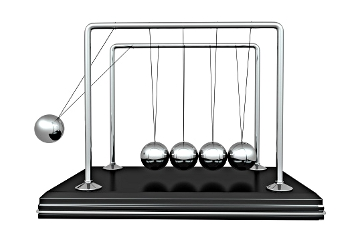
\includegraphics[width=0.5\linewidth]{2021-2/img/ejercicios/imagen_ej7_1.jpeg}
    \caption{Dispositivo de esferas idénticas.}
\end{figure}



\begin{figure}[H]
  \begin{subfigure}[b]{0.4\textwidth}
    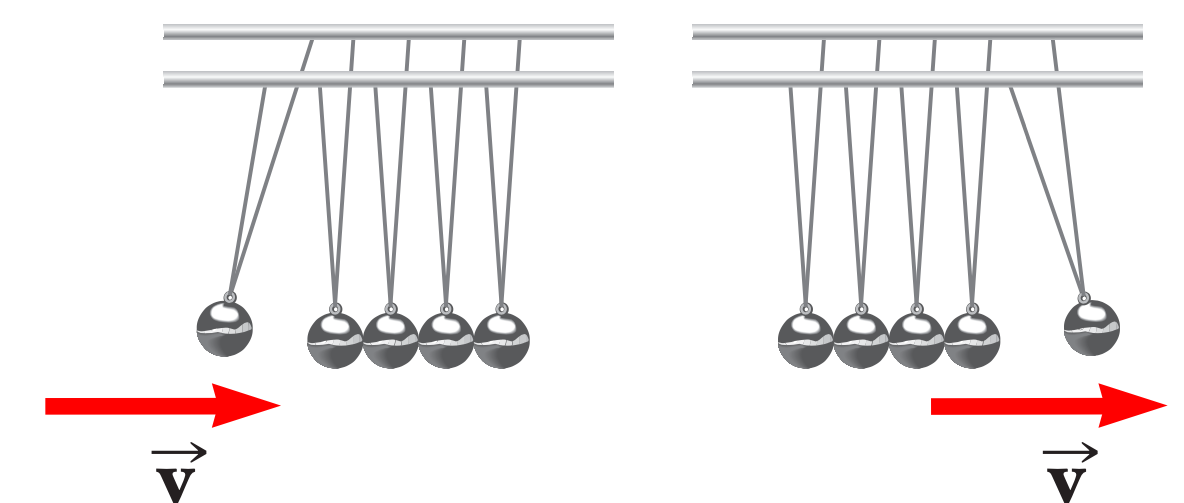
\includegraphics[width=\textwidth, height=0.55\textwidth]{2021-2/img/ejercicios/imagen_ej7_2.png}
    \caption{Puede ocurrir}
    \label{fig:f1}
  \end{subfigure}
  \hfill
  \begin{subfigure}[b]{0.4\textwidth}
    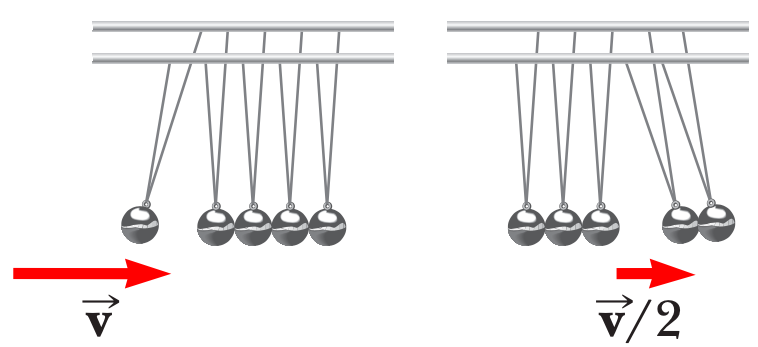
\includegraphics[width=\textwidth, height=0.56\textwidth]{2021-2/img/ejercicios/imagen_ej7_3.png}
    \caption{Puede ocurrir?}
    \label{fig:f2}
  \end{subfigure}
  \caption{(a) Situación observada. (b) Situación que se pide investigar factibilidad. }
\end{figure}




\end{enumerate}
\end{document}